\documentclass{article}

\usepackage{arxiv}

\usepackage[utf8]{inputenc} % allow utf-8 input
\usepackage[T1]{fontenc}    % use 8-bit T1 fonts
\usepackage{hyperref}       % hyperlinks
\usepackage{url}            % simple URL typesetting
\usepackage{booktabs}       % professional-quality tables
\usepackage{amsmath,amsfonts}       % blackboard math symbols
\usepackage{nicefrac}       % compact symbols for 1/2, etc.
\usepackage{microtype}      % microtypography
\usepackage{lipsum}
\usepackage{graphicx}
\usepackage{smartdiagram}

\title{Investigation of Quadratic Shaped Cantilever Beam Type Piezoelectric Energy Harvesters for Improved Harvesting Efficiency }


\author{
  Nezih Topaloglu\thanks{Use footnote for providing further
    information about author (webpage, alternative
    address)---\emph{not} for acknowledging funding agencies.} \\
  Department of Mechanical Engineering\\
  Yeditepe University University\\
 Istanbul, Turkey 34755 \\
  \texttt{nezih.topaloglu@yeditepe.edu.tr} \\
  %% examples of more authors
  \And
  C. Volkan Karadag \\
Department of Mechanical Engineering\\
  Yeditepe University University\\
 Istanbul, Turkey 34755 \\
  \texttt{volkaradag@gmail.com} \\
  \AND
  Seyda Ertarla \\
Department of Mechanical Engineering\\
  Yeditepe University University\\
 Istanbul, Turkey 34755 \\
  \texttt{seydaertarla@gmail.com} \\
  \And
 A. Fethi Okyar \\
Department of Mechanical Engineering\\
  Yeditepe University University\\
 Istanbul, Turkey 34755 \\
  \texttt{okyar@yeditepe.edu.tr} \\
  %% \And
  %% Coauthor \\
  %% Affiliation \\
  %% Address \\
  %% \texttt{email} \\
}

\begin{document}
\maketitle

\begin{abstract}
\lipsum[1]
\end{abstract}


% keywords can be removed
\keywords{First keyword \and Second keyword \and More}


\section{Introduction}
Research has increased on vibration energy harvesting in recent years. Applications of vibration energy harvesters (VEH) hold up as sensor networks, body sensor networks and portable electronic devices for today and future. Electromagnetism, electrostatics and piezoelectricity are methods which generate energy form vibration. 

Piezoelectric cantilever beam among vibration energy harvesting methods is trend topic. There is various research to increase efficiency of piezoelectric-based cantilever beam VEHs. Objective is to generate more energy by obtaining uniform stress distribution along the beam. However, many results aimed increase of stress distribution have been seen a small amount of improvement. In order to this, some solution proposals are not applicable to standard piezoelectric beams.

Research is concentrated on piezoelectric-based cantilever beam VEHs of late years. To exemplify, Ma et al attached to a compliant hinge mechanism at the tip of cantilever beam to improve stress distribution along beam. Proof mass is attached at the tip of the link. The compliant mechanism at the tip can increase the tip displacement, so it produces large motion of the proof mass[3].

A MEMS piezoelectric cantilevered vibration energy harvester on c-axis tilted AlN thin film was investigated by Kong et al. Effects of geometry parameters and c-axis tilted angle were examined. This method improves stress profile, but it is difficult to fabrication. 

Raju et al is the one of the researcher related to subject of cantilever piezoelectric energy harvesting. Raju developed a method which is piezoelectric energy harvester with multiple rectangular cavities at a single section and two sections. Result is found that maximum voltage is produced with two cavities and more voltage is generated with a single cavity section in comparison with two cavity sections [5].

Yoon et al also analysed optimization of curved piezoceramic unimorphs to generate more charge due to mechanical loading. PZT (lead zirconate titanate) unimorph structure is placed as horizontal in order to generate surface charge when vertically loaded and the charge can be collected, but in this methods, pressure load is applied on the top surface [6]. Therefore, it is not sufficient to generate energy from vibration. 

Models of piezoelectric energy harvesters with tapered unimorph cantilever beams extended proof mass were found out Halvorsen et al. Research embraces for long and short beam. In outcome study for tapering the beam exactly does not conclude to make more homogeneous stress and has not any performance advantage when these harvesters is optimized for single frequency [7]. 

Xiong et al is worked on tapered two-layer piezoelectric vibration energy harvesters. Base cantilever beams and upper cantilever beams are attached each other. Two masses also attached to each layer. The convergent and divergent tapered harvesters can generate about resonance frequencies by changing the positions of the masses [8]. 

Piezoelectric energy harvesting from trapezoidal bimorph piezoelectric cantilever beams with proof mass was worked on by Kianpoor et al. It is seen that geometrical parameters (width, thickness and length of beam and also the dimensions of proof mass) affect excessively harvester’s performance. Direct and reverse trapezoidal beams and rectangle beams are compared in term of energy obtained values. it is ensued that the reverse trapezoidal geometry can produce more electrical power and voltage than other geometries [9]. 

Recently, Roundy et al focused on importance of different piezoelectric beam shape. Tapered beam was suggested A trapezoidal geometry can provide more than twice the energy than the rectangular geometry. However, neither theoretical and experimental are worked [10]. 

Research is seen to rule out effect of tip mass and geometrical parameters. In below figure it is seen strain vs length graph for rectangular (a), triangle (b). There is energy improvement by varying from rectangular to triangle, so it is worked on optimized shape (c) which can be obtain more energy than other cantilever beams. In this study, it is aimed to obtain more energy by optimizing different beam geometries which shape by tip mass weight. Calculations obtained energy are made  from first 80 percent of beam length.In this paper, extensive analytic model and experimental results are presented.

\begin{figure}[ht!]
\centering
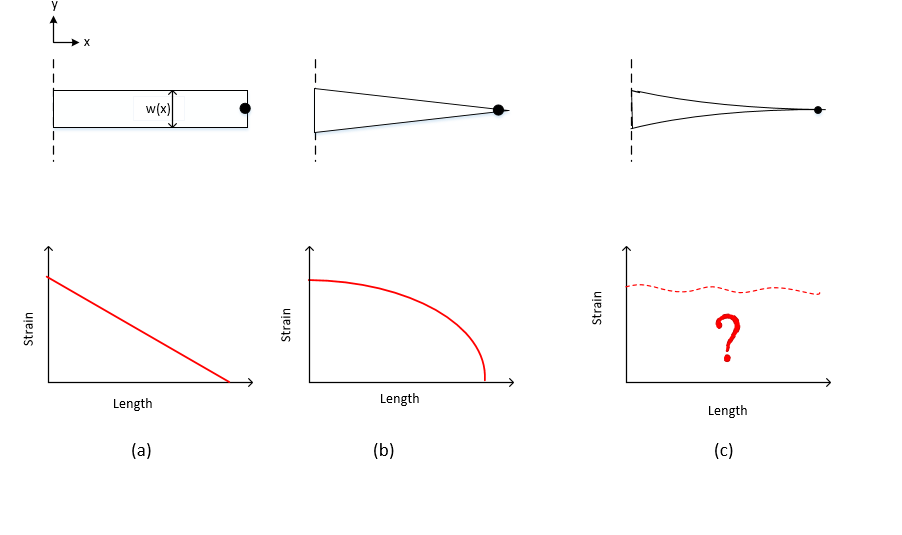
\includegraphics[width=90mm]{figures/graph.PNG}
\caption{ \label{overflow}}
\end{figure}
\label{sec intro}
\begin{itemize}

    \item SE and NT
    \item General paragraph on energy harvesting
    \item Beam type harvesters and the stress uniformity challenge
    \item Solutions offered so far:
    \item Ma 2016, Roundy 2005 and others
    \item The full text of the ICOVP 2019 Paper (Crete) may be useful
\end{itemize}

numerous works on well-known geometric shapes such as triangles, rectangles, etc., defining the contours/outlines used to generate cantilever beams exist.  However, other beams having arbitrary contour may well outperform the simple contours/outlines. In order to determine a best-in-class contour/outline optimization methods can be used in tandem with structural analysis approach.

definition:: \textbf{transverse plane} of the beam which contains both the axial as well as base-excitation direction. on which the contours are visible

\section{Theory}
In the finite-element method (FEM), the harmonic solution of linear problems are expressed in complex arithmetic, where the force term (or in case of base-excitation, the boundary term) is written as
\begin{equation}
    \mathbf{F} (t) = \mathbf{\hat F} (\omega) \exp(i\omega t)
\end{equation}
where $i=\sqrt{-1}$ and $\omega$ denotes the frequency of oscillations. The notation $(\hat{})$ is used for complex quantities. Thus, the complex force intensity may be separated into 
\begin{eqnarray}
 \mathbf{F}_r & = & \mathrm{Re}(\mathbf{\hat F}) \\
 \mathbf{F}_i & = & \mathrm{Im}(\mathbf{\hat F})
\end{eqnarray}
For a linear problem the mass, damping and stiffness matrices, respectively, $\mathbf{M}$, $\mathbf{C}$, and $\mathbf{K}$, are constant and a solution in the form
\begin{equation}
    \mathbf{u}(t) = \mathbf{\hat u}(\omega)\exp(i\omega t)
\end{equation}
that satisfies the equation of motion
\begin{equation}
    \left[ -\omega^2 \mathbf{M} + i \omega \mathbf{\hat C} + \mathbf{\hat K} \right] \mathbf{\hat u} =  \mathbf{\hat F} \label{eqn:motion}
\end{equation}
for each specified frequency and load is sought. In Rayleigh damping, the damping matrix is expressed as
\begin{equation}
    \mathbf{\hat C} = a_0 \mathbf{M} + a_1 \mathbf{\hat K}
\end{equation}

In this work, a research-type FEM package called FEAP \cite{feap} was used. The FEAP source code was modified in order to introduce Rayleigh damping into an existing shell element, as formulated above and outlined in \cite{taylor07}.

The above formulation is applicable, in general, for any type of finite element including beams and shells. Although our model is a beam, it has a large width/height ($b/h$) ratio to allow for patching. This results in warpage and non-uniform transverse displacements, rendering the beam theory ineffective, and requiring the use of two-dimensional models.  For that purpose, shell-type finite elements (FE) are employed instead of the beam-types. Shell elements are two-dimensional surface elements with a very low bending/membrane stiffness ratio\cite{bischoff}. 

The shell element formulation in FEAP is based on the discrete Kirchhoff quadrilateral formulation for plates \cite{batoz82a,taylor88}. In our model, harmonic base-excitation loading was applied under small displacements and complex arithmetic, details of which may be found in \cite{zienkiewicz}. 

%\section{Optimization based on Structural Analysis}
\section{Methodology}
\label{sec:fem_opt}
The methodology is depicted in Figure \ref{fig:method}. The three main activities involved are, 1) establishing a computational scheme for the solution and evaluating the beam response under base-excitation, 2) construction of an optimization loop that finds the optimal beam profile shape which yields a homogeneous surface strain distribution, and 3) validation of selected results from the previous step by experimentation.
\begin{figure}
    \centering
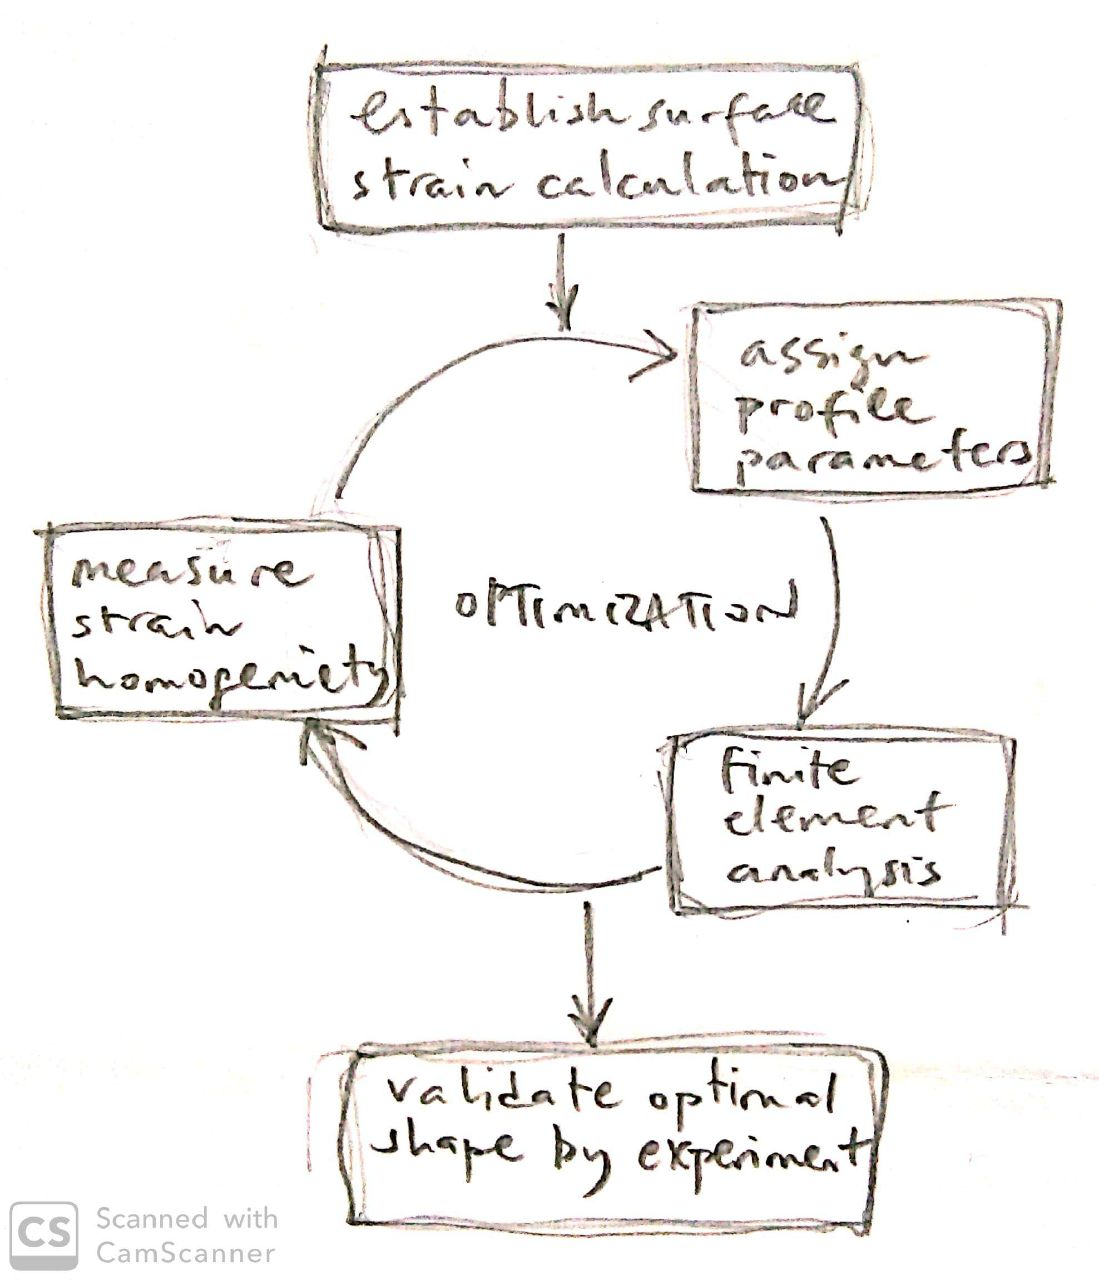
\includegraphics[width=.5\linewidth]{figures/metot-el}
    \caption{An overview of the methodology section}
    \label{fig:method}
\end{figure}

 Rectangular and triangular shaped beam models in Figure \ref{fig:basicmesh} were subjected to base-excitation in the out-of-plane direction. In FEAP, the matrices $\mathbf{M}$, $\mathbf{\hat C}$ and $\mathbf{\hat K}$ of Eq. \ref{eqn:motion} were obtained by assembling regular meshes of QUAD4-type elements shown in Figure \ref{fig:basicmesh}. 
 
 At first, the homogeneous form of Eq. \ref{eqn:motion}  using the parameters in Table \ref{tab:basicparams} was solved to obtain natural frequencies of vibration. These results are checked against the two-dimensional analytical plate solutions in Section \ref{sec:fem_results}.  
 
\begin{figure}
    \centering
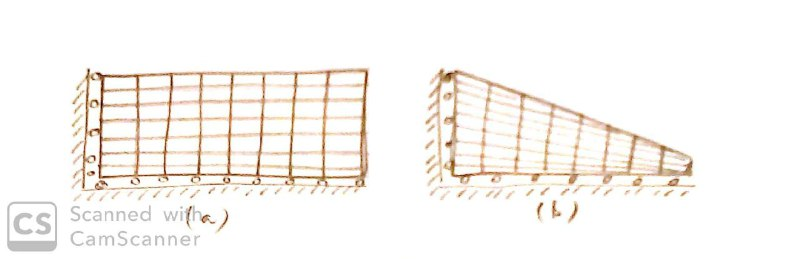
\includegraphics[width=\linewidth]{figures/basicmesh}
    \caption{Finite element half-meshes depicting basic shapes such as a rectangle (a) and a triangle (b). Base excitation is applied at the left boundary while symmetry condition is applied at the lower (horizontal) boundary.}
    \label{fig:basicmesh}
\end{figure}

\begin{table}
    \centering
    \begin{tabular}{|c|c|} \hline
        \parbox{.8in}{\centering MATERIAL} & 
        \parbox{.8in}{\centering GEOMETRY} \\\hline
        \parbox{.8in}{\centering Elastic\\Modulus} & 
        \parbox{.8in}{\centering Length} \\
        (Pa) & (m) \\\hline
        &  \\\hline\hline
        \parbox{.8in}{\centering Poisson's\\Ratio} &
        \parbox{.8in}{\centering Width\\(m)} \\\hline
        &  \\\hline\hline
        \parbox{.8in}{\centering Density}  &
        \parbox{.8in}{\centering Thickness} \\
        (kg/m$^3$) & (m) \\\hline
        &  \\\hline
    \end{tabular}
    \caption{Model parameters used in the determination of natural frequencies in the first step}
    \label{tab:basicparams}
\end{table}

Then the models in Figure \ref{fig:basicmesh} were subjected to base-excitation around their fundamental natural frequencies in order to obtain axial strain-distributions. Uniformity of the axial strain distribution was assessed by a so-called efficiency parameter, $\kappa$, defined as
\begin{equation}
    \kappa = \frac{\epsilon^{\mathrm{max}}_{xx}}{\epsilon^{\mathrm{ave}}_{xx}}
\end{equation}
where $\epsilon^{\mathrm{max}}_{xx}$ and $\epsilon^{\mathrm{ave}}_{xx}$ are the maximum and average values of the distribution, respectively.


The second step of methodology consisted of optimization aimed to increase the energy harvesting capacity by changing the beams width profile. Using the  computational framework to calculate the energy-harvesting efficiency parameter, $\kappa$, laid out in the first step, the main Matlab script; 1) generates an arbitrary width profile, 2) constructs it's corresponding mesh, 3) sends the mesh and an appropriate input file to FEAP, 4) grabs the FEAP output, 5) extracts the efficiency parameter $\kappa$ from the output, and 6) optimizes the width profile parameters, $a$ and $b$, for maximum efficiency. 

Optimization was carried out by finding the minimum of an unconstrained multivariable objective function using a derivative-free method, utilized by the \texttt{fminsearch} function in Matlab \cite{matlab}. 

\paragraph{explain} the variables, parameters defining the contour/outlines

\paragraph{morphing} a regular rectangular mesh into a four-edge shape with arbitrary contour

\section{Results of the Optimization}
\label{sec:fem_results}
At first, the surface strain distributions were obtained via finite element method (FEM) for a rectangle and a triangle. 

\begin{figure}[ht!]
\centering
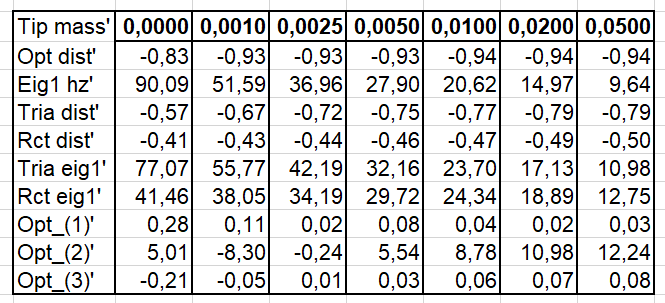
\includegraphics[width=90mm]{figures/tablo_prim.PNG}
\caption{ \label{overflow}}
\end{figure}

\begin{figure}[ht!]
\centering
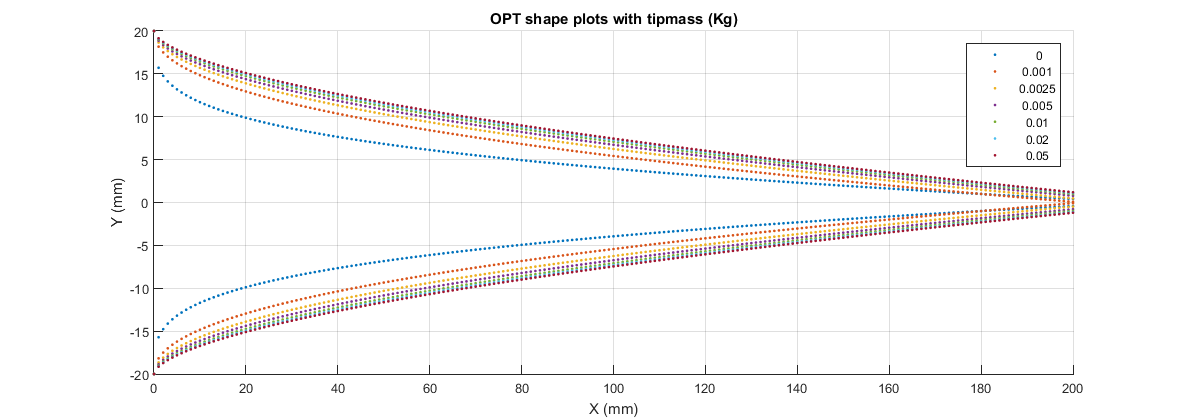
\includegraphics[width=90mm]{figures/opt_shapes.png}
\caption{ \label{overflow}}
\end{figure}

\begin{itemize}
    \item SE, CVK and FO
    \item Volkan's famous table
    \item Figures need to be finalized
    \item Important result: The optimal shape converges to triangular shape as the tip mass increases

\end{itemize}

\section{Experimental Verification}
\label{sec:exp_results}

To compare the stress distribution of an optimal beam with that of a triangular and rectangular beams, experiments are performed using a Permanent Magnet shaker. The Aluminum beams used in the experimental study can be seen in Fig. XXX. Six beams are produced: opt-0g, tri-0g, rec-0g, opt-5g, tri-5g and rec-5g. Their properties can be checked from Table XX of Section \ref{sec:fem_results}. The weights are fixed to the beam tip using epoxy.

\begin{figure}[ht!]
\centering
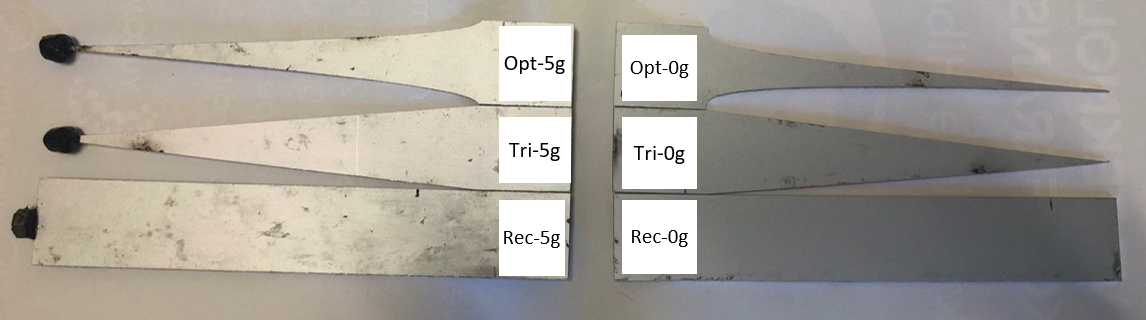
\includegraphics[width=90mm]{figures/6beams.PNG}
\caption{Photos of tested beam samples both with and without a tip-mass.}
\label{samples}
\end{figure}

The measurement of strain distribution on a beam surface is not straightforward. Preliminary measurements using a series of strain gauges showed that the strain gauges and their cables significantly affect the dynamics of the beam and the reliability of the results. Therefore, an indirect and non-contact method is applied. A laser displacement sensor is used to scan the beam surface during vibration. Scanning is performed from the beam base to its tip, along the beam's line of symmetry. To ensure smooth and precise scan, an in-house scanner mechanism is designed and built. The linear motion of the displacement sensor is ensured using a step motor with a power screw. A photograph of the scanner mechanism can be seen in Fig. XXX

The block diagram of the experimental setup is seen in Fig. XXX(a) and its photograph is given in  Fig.XXX(b). The beam is fixed from its base to the shaker. The laser displacement sensor is adjusted properly to perform the scan along the beam axis during vibration. The displacement signal is read using a data acquisiton (DAQ) system. The step motor is controlled using a step motor driver and Arduino microcontroller. The DAQ system and Arduino are connected to separate laptops to prevent electrical noise.

The experimental procedure is as follows: First, a frequency sweep is applied to the shaker and frequency response of the beam is recorded. From the peak response, the resonance frequency of the beam is determined. The beam is then oscillated at its resonance, while the sensor performs the axial scan. The recorded data is then filtered and a polynomial is fitted to the data set generated by the positive peaks of the displacement data.
By taking the second derivative of the fitted polynomial, the strain along the beam axis ($\epsilon(x)$) is found. The area-averaged strain is calculated as follows
\begin{equation}
\epsilon_{AA} = \frac{\int_{0}^{L}\epsilon \left ( x \right ) w\left ( x \right ) dx}{\int_{0}^{L} w\left ( x \right ) dx}
\end{equation}
where $w(x)$ is the width function. The denominator of the above equation corresponds to the beam surface area. Finally, the strain (or stress) distribution is calculated by dividing the area averaged strain to maximum strain.

\begin{figure}[ht!]
\centering
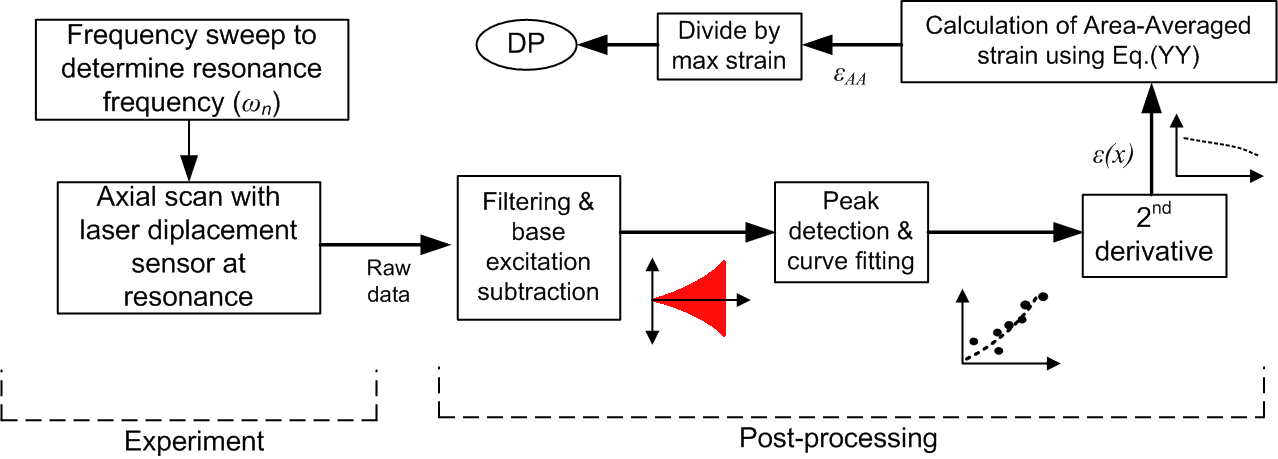
\includegraphics[width=120mm]{figures/exp_proc.png}
\caption{ \label{overflow}}
\end{figure}


\begin{itemize}
    \item CVK and NT
    \item Experimental setup.
    \item Results for no mass and 5 gr.
    \item Comparison of results among each other.
    \item Proving the idea
    \item Figures need to be finalized


\end{itemize}

\begin{figure}[ht!]
\centering
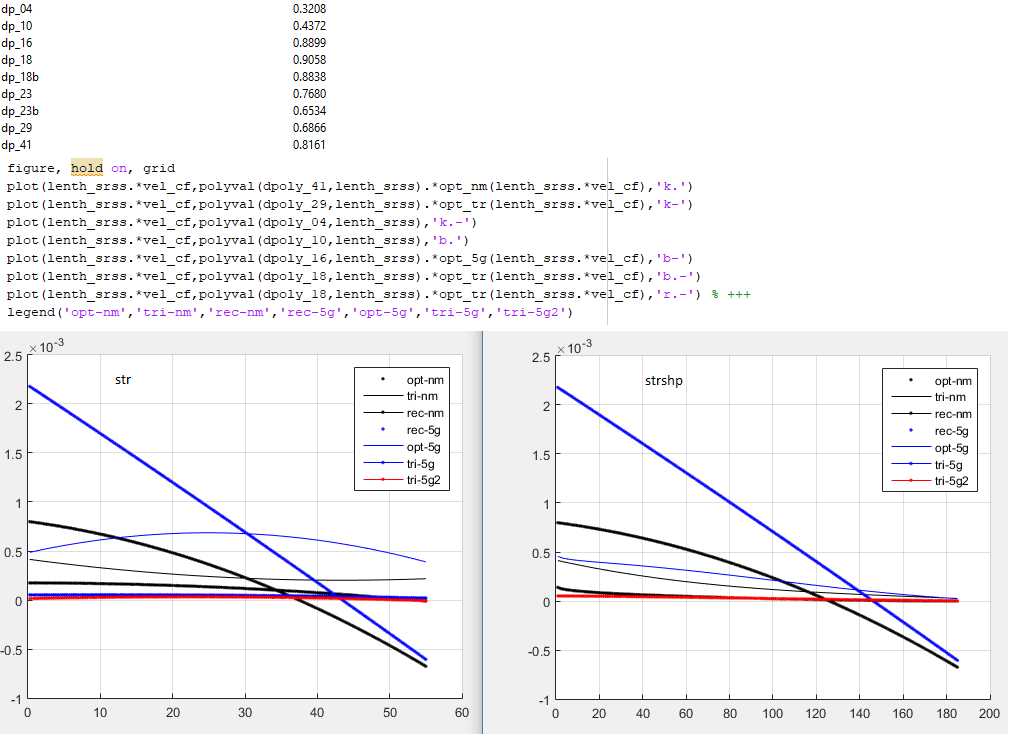
\includegraphics[width=90mm]{figures/adsiz.PNG}
\caption{ \label{overflow}}
\end{figure}
\label{sec intro}

\section{Discussion} 
The energy harvesting capacity of wide beams under base-excitation in their out-of-plane directions have been undertaken using FEM. The uniformity of axial strain distribution has fundamental implications over the energy harvesting capacity of beams. This capacity is directly proportional with the homogeneity of the axial strain distribution along the beam's lateral surfaces (the top and bottom surfaces)...



\section{Conclusion}

\bibliographystyle{unsrt}  
%\bibliography{references}  %%% Remove comment to use the external .bib file (using bibtex).
%%% and comment out the ``thebibliography'' section.


%%% Comment out this section when you \bibliography{references} is enabled.
\begin{thebibliography}{1}

\bibitem{}
N. Topaloglu, V. Karadağ and Ş. Ertarla.
\newblock Analytical Modeling of a Cantilever Beam Type Vibration Energy Harvester with a Lever Mechanism.
\newblock In {\em International Conference on Noise and Vibration Engineering, 2018 ISMA-USD Conference}, pages ???. 2018.

\bibitem{}
N. Topaloglu, V. Karadağ and Ş. Ertarla.
\newblock Axial and transverse vibration of a cantilever beam energy harvester with a tip mass with axial and transverse eccentricity.
\newblock In {\em 14th International Conference on Vibration Problems, 2019 Icovp}, pages ???. 2019.

\bibitem{}
X. Ma, A. Wilson, C.D. Rahn and  S. Trolier-McKinstry.
\newblock Efficient Energy Harvesting Using Piezoelectric Compliant Mechanisms: Theory and Experiment.
\newblock {\em Journal of Vibration and Acoustics, Vol. 138, No. 2, pp. 21005,}, 2016.

\bibitem{}
L. Kong, J. Zhang, H. Wang, S. Ma, F. Li, Q.-M. Wang and L. Qin.
\newblock Simulation study of MEMS piezoelectric vibration energy harvester based on c-axis tilted AlN thin film for performance improvement.
\newblock {\em Journal of Vibration and Acoustics, Vol. 138, No. 2, pp. 21005}, 2016.

\bibitem{}
S.S. Raju, M. Umapathy and G. Uma.
\newblock Cantilever piezoelectric energy harvester with multiple cavities.
\newblock {\em Smart Material Structure, IOPSCIENCE, Vol. 24, No. 11, pp. 115023}, 2015.

\bibitem{}
H.S. Yoon, G. Washington and A. Danak.
\newblock Optimization, and Design of Efficient Initially Curved Piezoceramic Unimorphs for Energy Harvesting Applications.
\newblock {\em Journal of Intelligent Material Systems and Structures, Vol. 16, No. 10, pp. 877-888},2015

\bibitem{}
E. Halvorsen and T. Dong.
\newblock Analysis of Tapered Beam Piezoelectric Energy Harvesters.
\newblock {\em Proceedings of PowerMEMS, pp. 241-244}, 2017.

\bibitem{}
X. Xiong and S. Olutunde Oyadiji.
\newblock Tapered Two-Layer Broadband Vibration Energy Harvesters. 
\newblock {\em Journal of Vibration and Acoustics,Vol. 137, No. 3, pp. 31011-31014}, 2015.

\bibitem{}
 A. Kianpoor and K. Jahani.
\newblock Modeling and Analyzing of Energy Harvesting from Trapezoidal Piezoelectric Beams.
\newblock {\em Iranian Journal of Science and Technology, Vol. 43, No. 1, pp. 259-266}, 2015.

\bibitem{}
S. Roundy, E.S. Leland, J. Baker, E. Carleton, E. Reilly, E. Lai, B. Otis, J. M. Rabaey, and P. K. Wright.
\newblock Improving power output for vibration-based energy scavengers.
\newblock {\em IEEE Pervasive Computing, Vol. 4, No. 1}, 2005.

\bibitem{feap}
R.L. Taylor.
\newblock{{FEAP} - Finite Element Analysis Program, v8.5 User Manual}, http://www.ce.berkeley/feap, accessed on Aug,1,2017.

\bibitem{bischoff}
M. Bischoff, K.-U. Bletzinger, W. A. Wall, and E. Ramm.
\newblock{Models and Finite Elements for Thin-Walled Structures in \emph{Encyclopedia of Computational Mechanics}}, Ch.3, 2014. 
\newblock{DOI:10.1002/0470091355.ecm026}

\bibitem{batoz82a}
J. L. Batoz and M.B. Tahar.
\newblock{Evaluation of a new quadrilateral thin plate bending element},
\newblock{\em Int Jour Num Meth Engng}, Vol.18, pp.1655--1677. (1982) 

\bibitem{taylor88}
R. L. Taylor
\newblock{Finite Element Analysis of Linear Shell Problems}
\newblock{\em The Mathematics of Finite Elements and Applications VI,
J. R. Whiteman, editor, Academic Press.} (1988)

\bibitem{zienkiewicz}
O. C. Zienkiewicz and R. L. Taylor
\newblock{The Finite Element Method for Solid and Structural Mechanics, 7ed}
\newblock{\em Elsevier Science.} (2013)

\bibitem{taylor07}
R. L. Taylor
\newblock{\em FEAP -- Complex Solutions}
\newblock{URL: \url{http://feap.berkeley.edu/forum/index.php?action=dlattach;topic=1801.0;attach=1996}, accessed Aug 11,2019.}


\end{thebibliography}

\end{document}